\documentclass{article}
\usepackage[utf8]{inputenc}
\usepackage{parskip}
\usepackage{graphicx}
% image path
\graphicspath{{./images/}}


\title{Documento di specifica software per il progetto di Ingegneria del Software Avanzata\par
    \textit{Progetto:} \textbf{ISA Blog}\\}

\author{Jipwouo chiege planck anders}
\date{}

\begin{document}

\maketitle
\clearpage

\tableofcontents
\clearpage

\section{Introduzione}
\label{sec:introduzione}

In questo documento si riportano le specifiche software di un servizio web ISA Blog.

\section{Requisiti}
\label{sec:requisiti}

\subsection{ISA Blog}

In primis, il compito dell'applicazione è quello di mettere a contatto gli studenti, gli insegnanti o gente di tutti
orrizonti, per condividere le loro esperienze e conoscenze.\\

Di ogni utente, l'applicazione deve memorizzare al autenticazione basato su provider OAuth (Google, GitHub)
e la registrazione tramite email (magic link):
\begin{itemize}
    \item il \textbf{nome utente}
    \item l'\textbf{immagine} del profilo
    \item l'\textbf{indirizzo email}
    \item la \textbf{password} (crittografata)
    \item il \textbf{ruolo} (utente o amministratore)
    \item il \textbf{provider} (Google, GitHub, email)
    \item il \textbf{token} di autenticazione
    \item la \textbf{data} e l'\textbf{ora} di creazione
    \item la \textbf{data} e l'\textbf{ora} di ultima modifica
\end{itemize}

L'applicazione deve offrire la funzionalità a degli \textbf{utenti registrati}
di poter aggiungere nuovi posts e interagire (commentare, like, bookmark) con i posts esistenti.

Di ogni post, l'applicazione deve memorizzare:
\begin{itemize}
    \item il \textbf{titolo}
    \item il \textbf{contenuto}
    \item la \textbf{data} e l'\textbf{ora} di creazione
    \item l'\textbf{autore} (nome utente, immagine profilo, ecc.)
    \item il \textbf{numero di like}
    \item il \textbf{numero di commenti}
    \item il \textbf{numero di bookmark}
    \item la \textbf{categoria} (es. informatica, matematica, fisica, ecc.)
    \item l'\textbf{immagine} di copertina
    \item l'\textbf{immagine} del post
\end{itemize}

ogni post può avere uno o più commenti e l'applicazione deve memorizzare:
\begin{itemize}
    \item il \textbf{contenuto} del commento
    \item la \textbf{data} e l'\textbf{ora} di creazione
    \item l'\textbf{autore} (nome utente, immagine profilo, ecc.)
    \item il post a cui si riferisce
\end{itemize}

ogni like è associato ad un post e all'utente che ha messo il like.\\
ogni bookmark è associato ad un post e all'utente che ha messo il bookmark.


\subsection{Isa Blog API base on supabase}

L'applicazione deve usufruire di un database PostgreSQL e di un serverless backend Supabase.
L'applicazione deve offrire delle REST API per poter ottenere per ogni risorsa:

profile (utente):
\begin{itemize}
    \item in base all'ID dell'utente (GET)
    \item in base all'ID dell'utente (PUT)
    \item in base all'ID dell'utente (DELETE)
\end{itemize}

posts:
\begin{itemize}
    \item la lista di tutti i posts (GET) con i relativi commenti, like e bookmark associati ad anche il profilo dell'autore associato
    \item in base all'ID del post (GET) con i relativi commenti, like e bookmark associati ad anche il profilo dell'autore associato
    \item in base ai dati del post (POST) (titolo, contenuto, categoria, immagine di copertina, immagine del post)
\end{itemize}

comments:
\begin{itemize}
    \item la lista di tutti i commenti (GET) con il profilo dell'autore associato
    \item in base ai dati del commento (POST) (contenuto, post a cui si riferisce)
\end{itemize}

likes:
\begin{itemize}
    \item un base all'ID del post (GET) con il profilo dell'autore associato al like
    \item toggle like (POST) in base all'ID del post (like/unlike)
\end{itemize}

bookmarks:
\begin{itemize}
    \item un base all'ID del post (GET) con il profilo dell'autore associato al bookmark
    \item toggle bookmark (POST) in base all'ID del post (bookmark/unbookmark)
\end{itemize}

Per ogni query $s$ ad nostro server db, l'applicazione deve restituire un JSON con i dati richiesti e un codice di stato HTTP:
\begin{itemize}
    \item \textbf{200 OK} se la query è andata a buon fine
    \item \textbf{400 Bad Request} se la query non è corretta
    \item \textbf{401 Unauthorized} se l'utente non è autenticato
    \item \textbf{403 Forbidden} se l'utente non ha i permessi per eseguire la query
    \item \textbf{404 Not Found} se la risorsa richiesta non esiste
    \item \textbf{500 Internal Server Error} se c'è un errore interno al server
\end{itemize}

Ogni query $s$ deve essere autenticata con un token JWT.

In particolare l'interfaccia web deve permettere di visualizzare
la lista dei posts, in particolare:
\begin{itemize}
    \item il titolo del post (con un link al post)
    \item l'immagine di copertina del post
    \item il numero di like
    \item il numero di commenti
    \item il numero di bookmark
    \item la categoria del post
    \item l'autore del post
    \item la data di creazione del post
    \item il overview del contenuto del post
    \item bottoni per mettere like, commentare e bookmark
\end{itemize}

L'eticchetta dello stato dell'icona like, commento e bookmark deve essere:
\begin{itemize}
    \item sempre \textbf{blue} per l'icona del commento (sempre attiva) numero di commenti.
    \item \textbf{giallo} se il post è stato salvato dall'utente registrato
    \item \textbf{rosso} se il post è stato likato da l'utente registrato
\end{itemize}

L'applicazione deve offrire inoltre delle REST API per poter ottenere:
\begin{itemize}
    \item la lista degli endpoint nel sistema con il loro stato
    \item la lista degli endpoint attivi
    \item un endpoint specifico con il suo stato (conoscendone l'URL)
\end{itemize}

\subsection{User management}

Per utilizzare l'applicazione e visualizzare lo stato degli endpoint è necessario disporre di un account utente.
L'interfaccia web deve permettere di registrarsi, di effettuare il login e di effettuare il logout.

Per ogni utente, l'applicazione deve memorizzare:
\begin{itemize}
    \item il \textbf{nome utente}
    \item l'\textbf{immagine} del profilo
    \item l'\textbf{indirizzo email}
    \item il \textbf{provider} (Google, GitHub, email)
    \item il \textbf{numero di telefono}
    \item il \textbf{mestiere} (default: viewer)
\end{itemize}

Un utente registrato sulla piattaforma può aggiungere nuovi posts e interagire con i posts esistenti.

\clearpage
\section{Data flow diagram}
\label{sec:data_flow_diagram}


\begin{figure}[h]
    \centering
    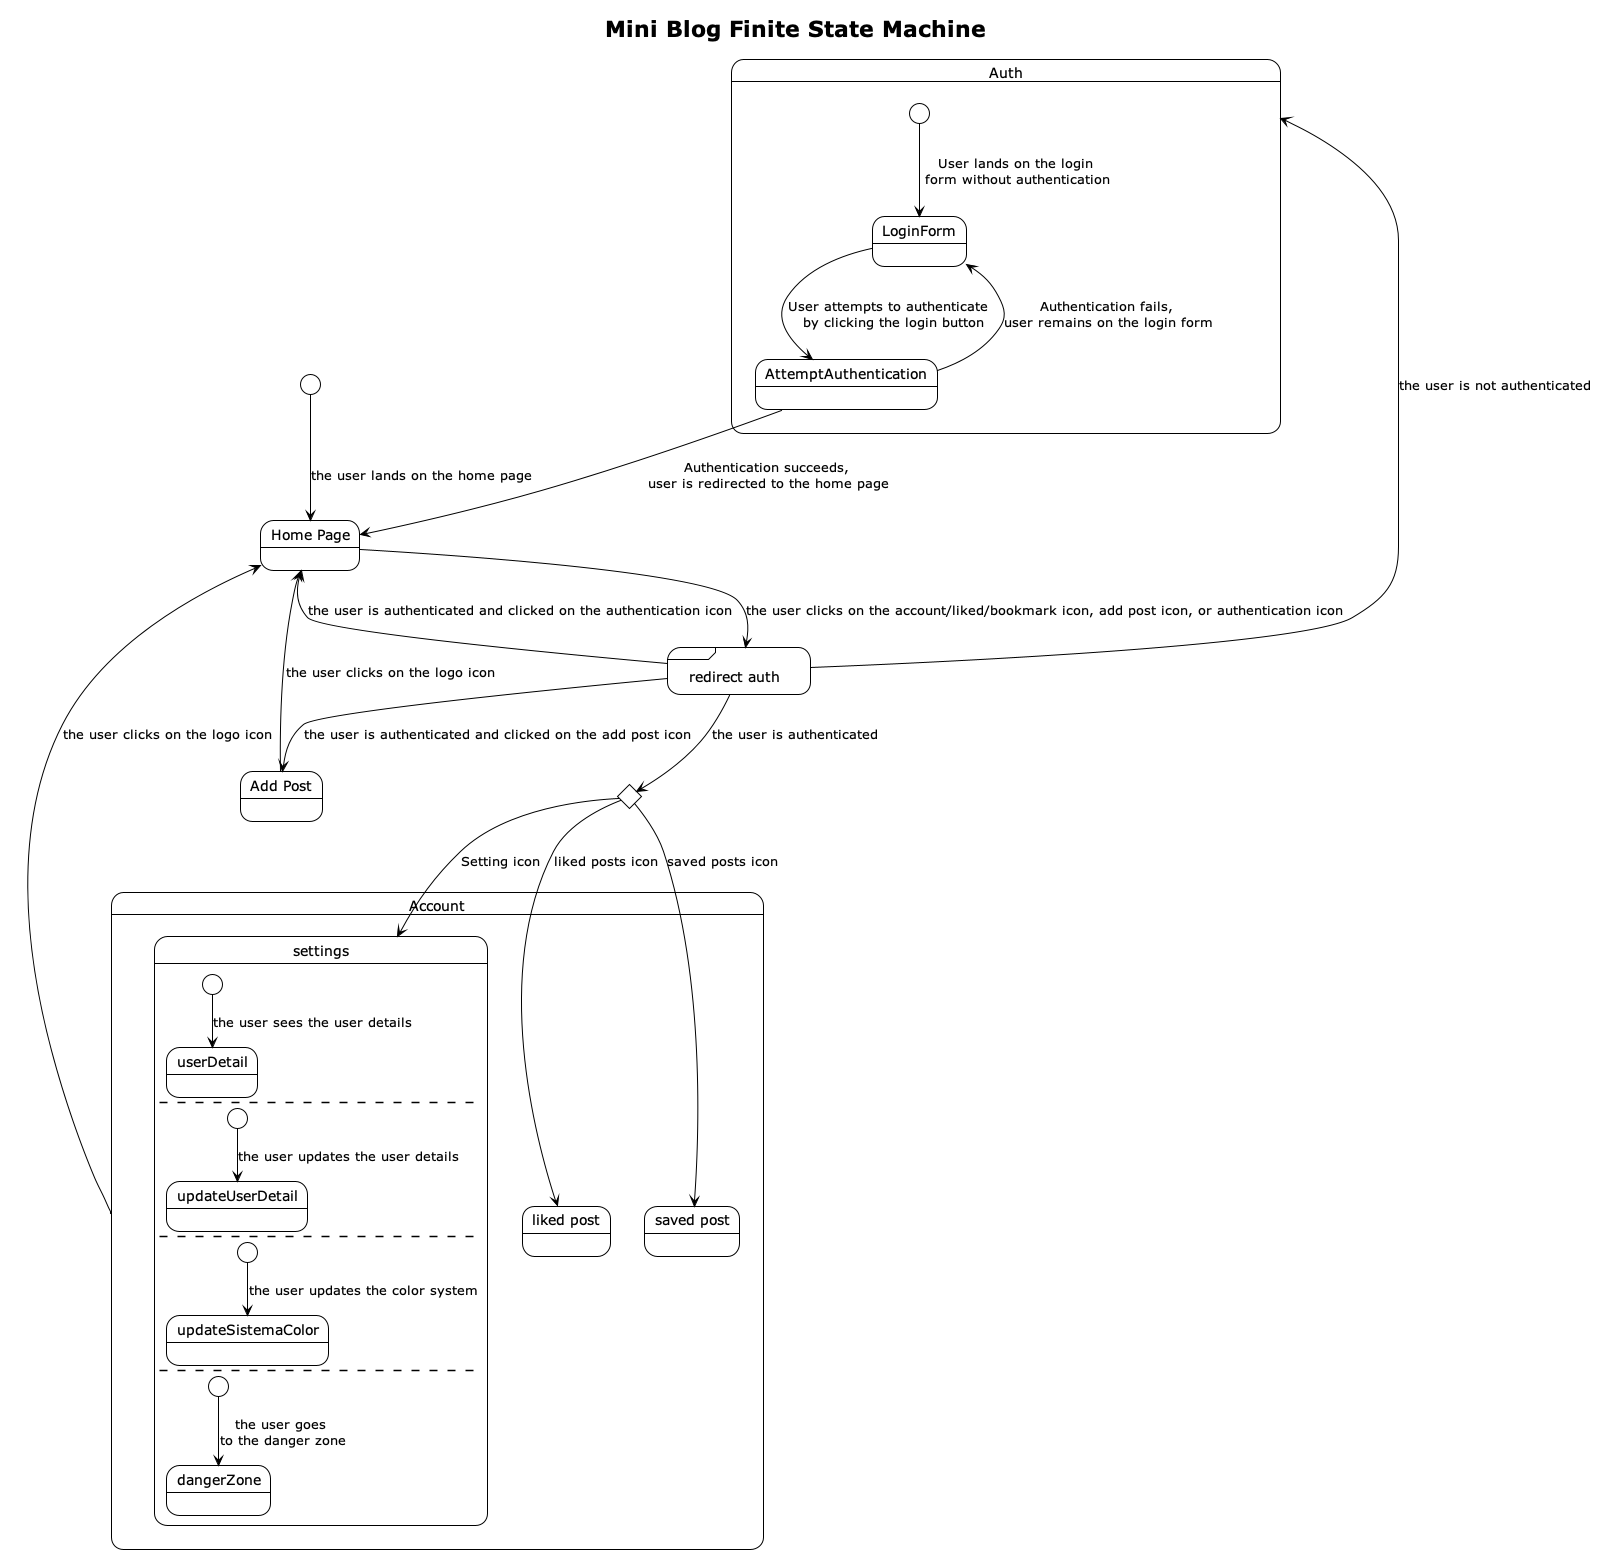
\includegraphics[width=1.3\textwidth]{ingblog_flow}
    \caption{ISA Blog flow}
\end{figure}

%raffinameto di administration
\begin{figure}[h]
    \lefting
    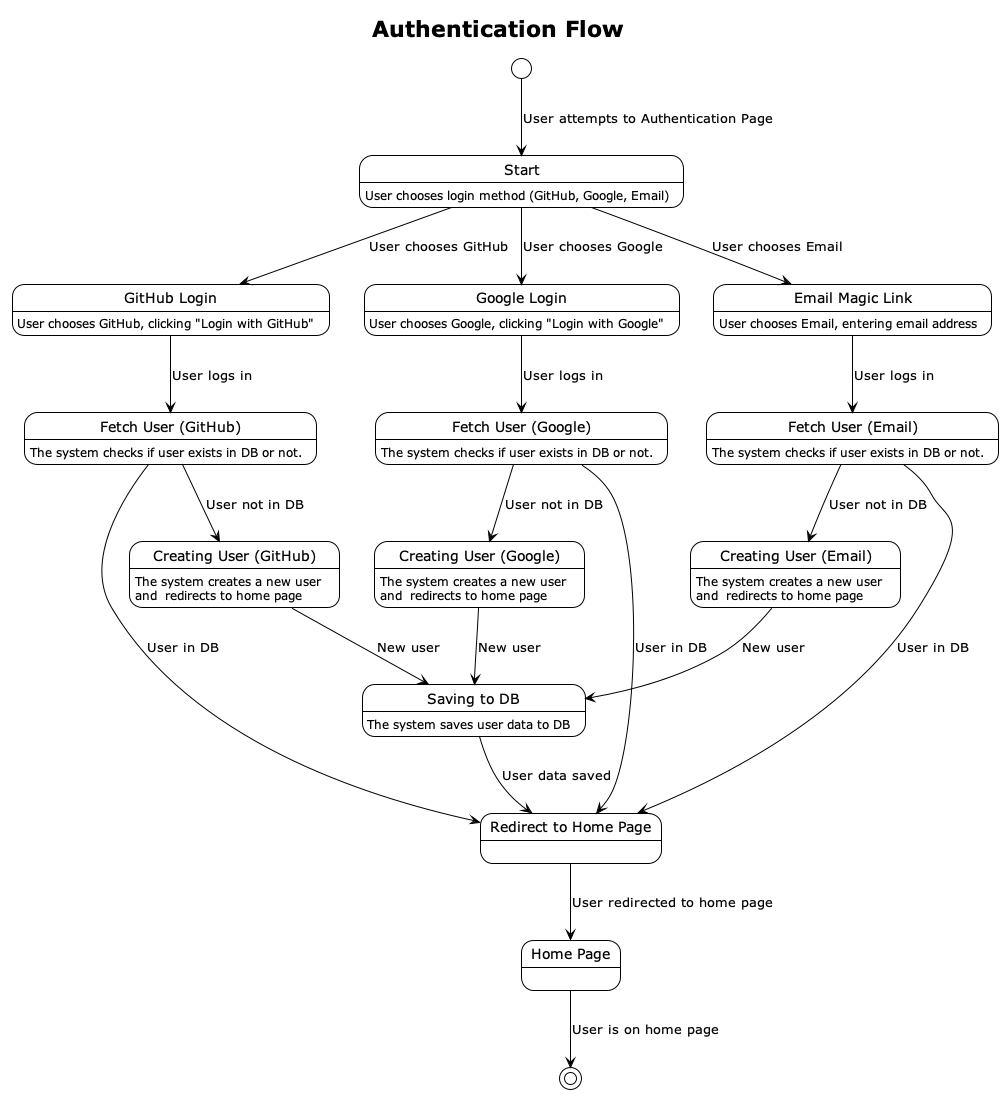
\includegraphics[width=1.3\textwidth]{authentication_flow}
    \caption{autenticazione flow}
\end{figure}

%raffinameto di sparql endpoint status reporting
\begin{figure}[h]
    \lefting
    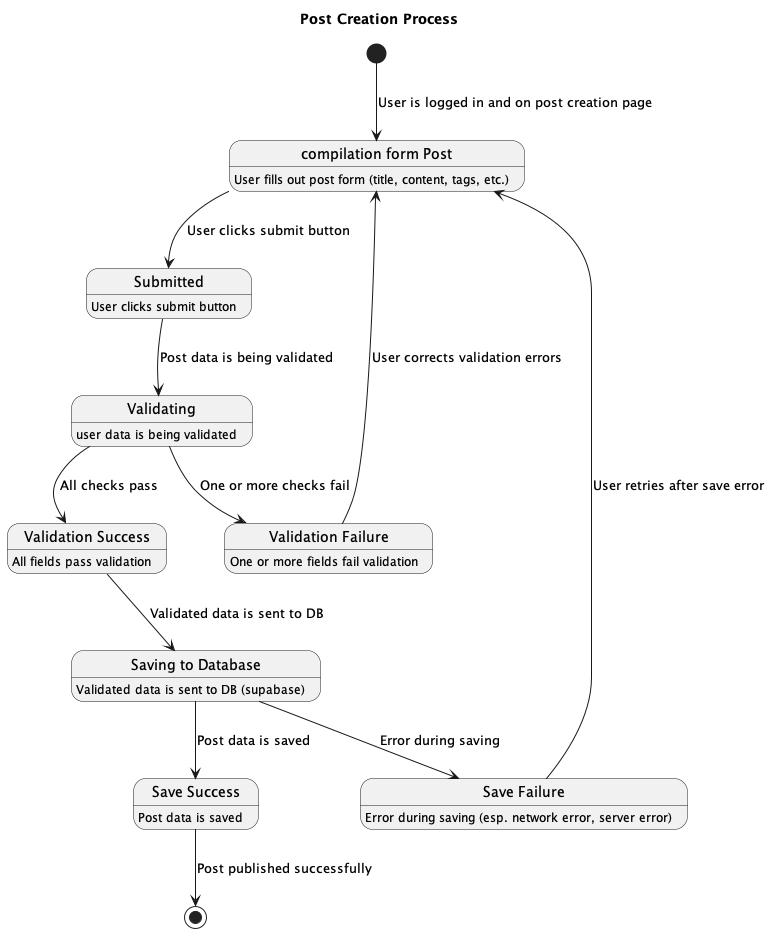
\includegraphics[width=1.3\textwidth]{creazione_post_flow}
    \caption{creazione post}
\end{figure}

\begin{figure}[h]
    \lefting
    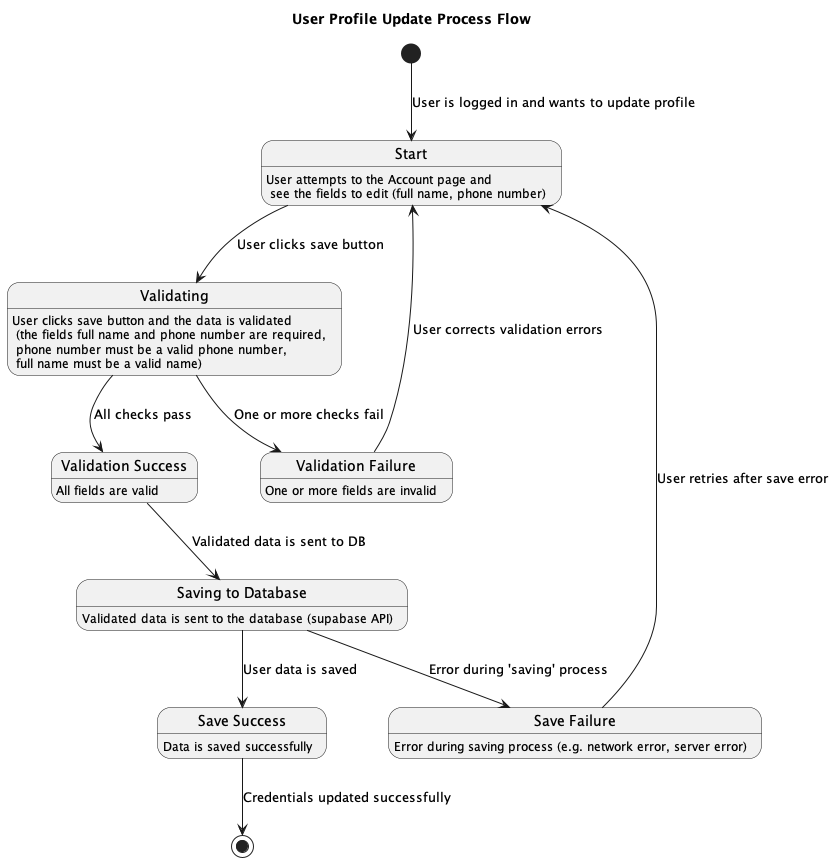
\includegraphics[width=1.3\textwidth]{modifica_profilo_flow}
    \caption{modifica profilo}
\end{figure}

\begin{figure}[h]
    \lefting
    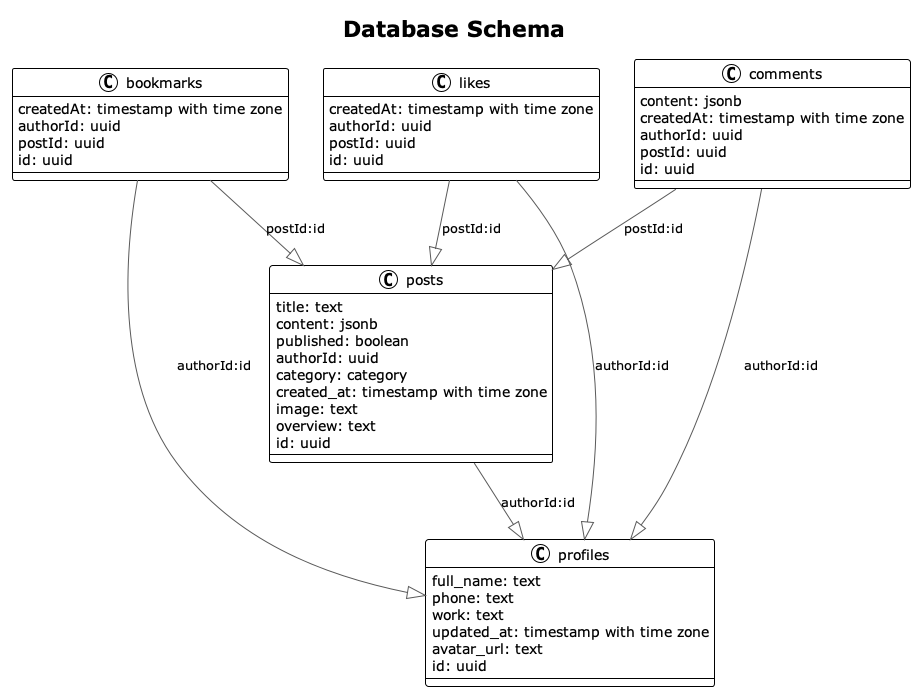
\includegraphics[width=1.3\textwidth]{database}
    \caption{database rapresentazione}
\end{figure}

\end{document}


